This section discusses the experimental setup and procedure, along with the calculation of the necessary quantities and their error analysis. 

To begin with, a class 3B external cavity diode laser (TuiOptics, DL100) emitting light of wavelength 987 mm is used for the experiment. A shutter mounted onto the laser controls the beam and a pair of anamorphotic prisms is used to modify the elliptical beam profile to a more circular shape. The laser, shutter and prism pairs were all fixed on a laser table beforehand. For each part of the experiment, other instruments and optical elements were added onto this setup.

\section{Variation of fundamental laser output power with injection current}
The first part of the experiment is aimed at familiarizing oneself with the dependence of the fundamental output power of the laser with the injection current and to extract various important parameters characterizing the laser such as the threshold current, differential slope efficiency and the differential quantum efficiency. 

In order to perform this experiment, a power meter was mounted on table in such a manner that it remains at the same height as that of laser beam as well as aligned with the beam (i.e. the face of the power meter is perpendicular to the beam axis). This adjustment was first performed by using an IR (infrared) detection card in order to ensure that the entire beam went into the power meter. Then the power meter is switched on, and the wavelength to be measured by it is set to 987 nm. Subsequently, finer adjustment is performed by moving the power meter to a position where it gives the maximum power reading. The power meter is then screwed tight at this position.

\begin{figure}[H]
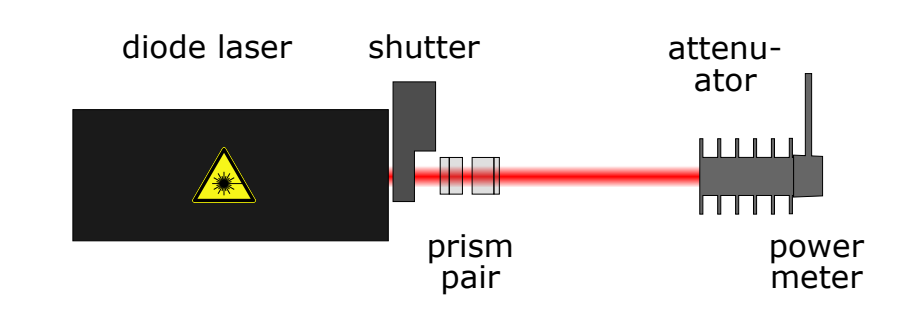
\includegraphics[scale=0.4]{./imagesandplots/pic1.png}
\centering
\caption{Set up to measure variation of laser output power with injection current \cite{UB}}
\label{figexpt1}
\end{figure}

The set up for this experiment (along with attenuator attached) is shown in Figure \ref{figexpt1}. With this setup in place, the injection current is increased from 0 to 280 mA in increments of 5 mA, and the corresponding values of output power are noted. Since the power meter sensor becomes non-linear for powers above 20 mW, it becomes necessary to use an attenuator. For our measurements, we took measurements both with and without attenuator in the unattenuated power range from 28.2 $\mu$W to 19000 $\mu$W (19 mW). Both the unattenuated and attenuated power values are necessary to be recorded over at least some data points in order to perform the calibration and extract a calibration factor from it. Beyond this range, the power is only measured with the attenuator attached onto the power meter, due to the aforementioned reason of non-linearity of the sensor. The attenuator for the experiment is a `1000:1' attenuator (meaning that ideally it would reduce the unattenuated power by a factor of 1000). The recorded data can be found in \ref{tab1}. The values measured without attenuator are listed under the column `$P_{unatt}$' and the measured power values with attenuator are under the column `$P_{att}$'. From now on, all errors stated in the tables should be assumed to be instrumental errors (least count of the measuring instrument), unless otherwise stated.

\subsubsection{Calibration of removable attenuator}
In order to find the calibration factor, the data for the attenuated power vs. unattenuated power is plotted and a linear fit is applied to this dataset. To carry out the curve fitting procedure using the data points and some initial guess parameters, we used the function \texttt{curve\_fit()} from the \texttt{scipy.optimize} module for \textit{Python}. The data points (along with x-y error bars) and the linear fit modelled onto them is shown in Figure \ref{figexpt2}.

\begin{figure}[H]
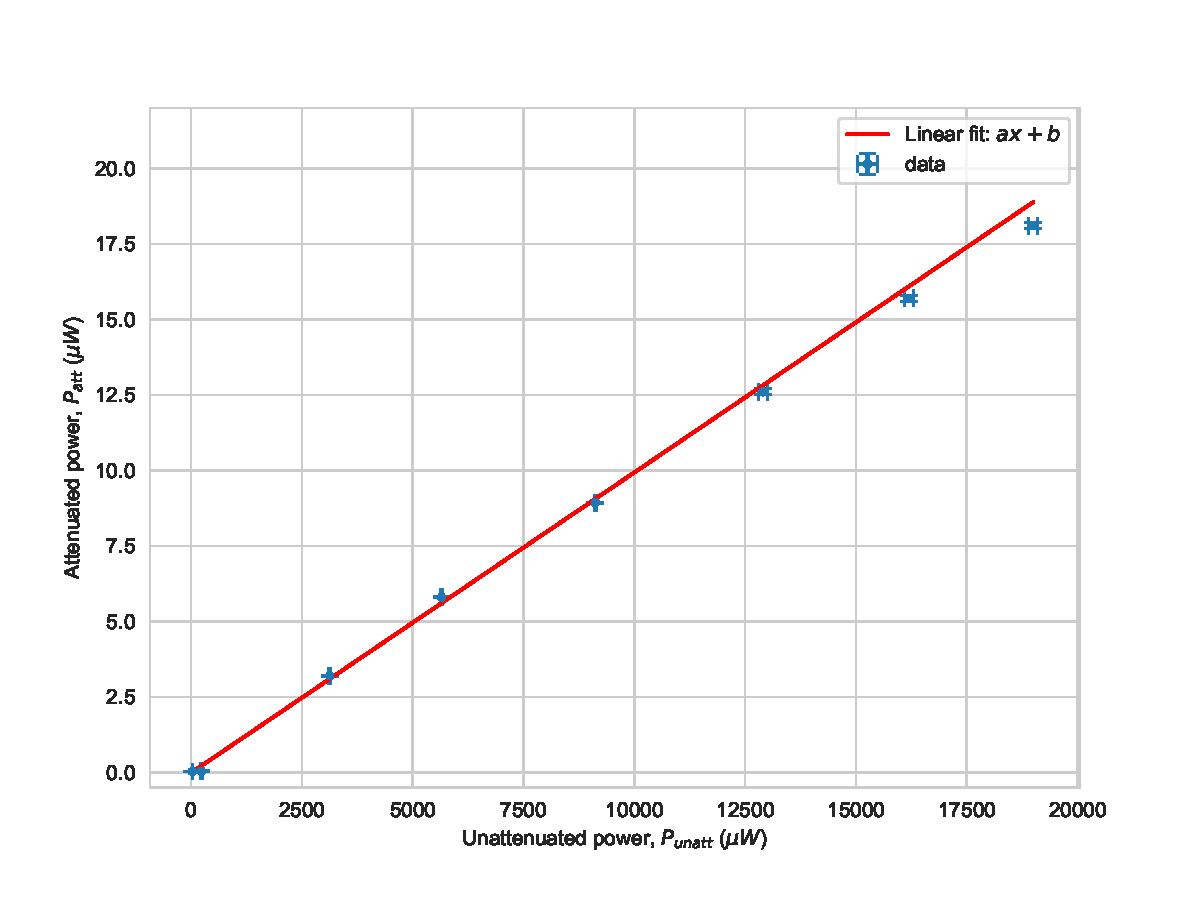
\includegraphics[width=0.9\textwidth]{./imagesandplots/attvsunattcalib.pdf}
\centering
\caption{Calibration plot of attenuated output power vs unattenuated power}
\label{figexpt2}
\end{figure}

The linear fit chosen is of the form: 
\begin{equation}
P_{att}=aP_{unatt}+b
\end{equation}

The choice of the initial guess parameters is taken as $a=0.001$ (since as already mentioned before, attenuated power is around 1/1000 of the unattenuated power, due to use of `1000:1' attenuator) and $b=0$ (y intercept expected to be a very small value, by visually extrapolating the data points). Indeed, after running the curve fitting procedure, we get fit parameters close to our initial guess: $a=0.000994\pm 1.25\times 10^{-6}$ and $b=-0.016\pm 0.006$, giving: $$P_{att}=(0.000994\pm 1.25\times 10^{-6})P_{unatt}+(-0.016\pm 0.006)$$
Now we use the commonly applied reduced $\chi^{2}$ test, to find the goodness of fit for this linear model: 
\begin{equation}
\chi^{2}=\sum_{i}\left[\dfrac{y_{i}(x_{i})-f_{i}(x_{i};p)}{\sigma_{i}}\right]^{2}
\end{equation}
where $y_{i}(x_{i})$ are the recorded y values (attenuated power in this case), $f_{i}(x_{i};p)$ is are y values from the fitting function with $p$ parameters (in this case the linear fit function with parameters $a$ and $b$).

Surprisingly, we get an extremely large reduced $\chi^{2}$ value of 174.69. 